\documentclass[10pt,a4paper]{article}
\usepackage[latin1]{inputenc}
\usepackage{amsmath}
\usepackage{amsfonts}
\usepackage{amssymb}
\usepackage{graphicx}
\usepackage{listings}
\usepackage[left=2cm,right=2cm,top=2cm,bottom=2cm]{geometry}
\author{Per Lenander, Anton Fosselius}
\title{ORGFX - getting started}

\begin{document}

\maketitle

\section{Introduction}
This document is intended to make it easier to get started with the ORSoC graphics accelerator component. It contains some useful links and instructions on how to get the example code working.

\newpage

\section{Project structure}

The project source is structured as seen in figure \ref{fig:directory}.

\begin{figure}
\begin{center}
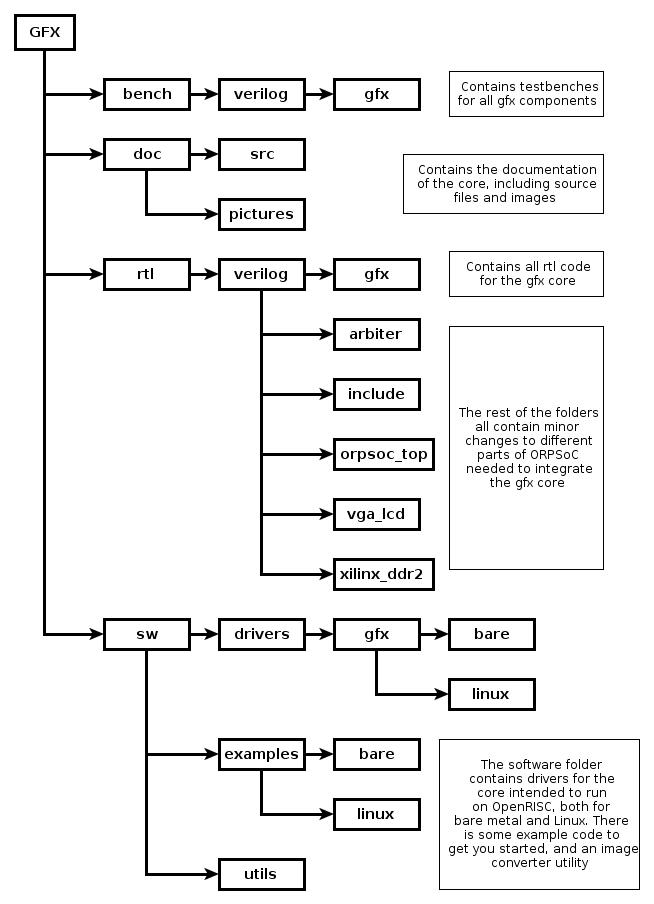
\includegraphics[scale=0.5]{../pictures/directory}
\caption{Directory structure of the ORSoC graphics accelerator.}
\label{fig:directory}
\end{center}
\end{figure}

\section{Hardware}
The \textbf{rtl} folder contains all the code needed to instantiate the ORGFX IP Core.

The component has 3 main wishbone interfaces:

\begin{itemize}
\item A wishbone slave interface for reading and writing registers. Every registry write will be added to a circular FIFO instruction queue.
\item A wishbone master interface for reading from memory (requires at least a read-only memory).
\item A wishbone master interface for writing to memory (requires at least a write-only memory).
\end{itemize}

All functionality of the component is accessed by writing instructions to the registers. Only writes to the control register can potentially start drawing operations.

Refer to the specification document for a full explanation of all registers, their default values and how they are used.

The component can be modified to extend the size of the instruction queue by changing the \textit{fifo\_depth} parameter. It is not advised to change the other parameters, as their function is not fully tested.

\section{Software}
\subsection{Drivers}
ORGFX comes with a layered software driver in the \textbf{sw/drivers} folder.

The basic driver consists of:

\begin{lstlisting}
orgfx.h
orgfx.c
orgfx_regs.h
\end{lstlisting}

It is possible to set the base bus address of the graphics accelerator in the regs file. The \textbf{orgfx.c} file is the only part of the driver that can interact with the hardware.

The extended driver (convenience functions and better surface management) consists of:

\begin{lstlisting}
orgfx_plus.h
orgfx_plus.c
\end{lstlisting}

The extended driver is required for most of the advanced API. Memory is managed statically in the driver, so the driver must be modified if support for a larger number of surfaces is desired.

There are four sets of advanced API that all build on the functionality of the basic and the extended driver:

\begin{lstlisting}
orgfx_3d.h
orgfx_3d.c
orgfx_tileset.h
orgfx_tileset.c
orgfx_bitmap_font.h
orgfx_bitmap_font.c
orgfx_vector_font.h
orgfx_vector_font.c
\end{lstlisting}

These supply convenience functions for doing more complex operations in a small number of function calls (such as drawing a 3D mesh). Most of these should be used with the output of the \textit{utilities} described below.

\subsection{Examples}
In addition to the drivers, the \textbf{sw} folder contains \textbf{examples}  and \textbf{utils}. The examples contain a few sample implementations with some basic functionality. The examples can be built by using the supplied Makefile. By default it builds the examples for hardware (requires or32-elf- toolchain to build for OpenRISC. The Makefile assumes that the or32-elf tool \textbf{bin2binsizeword} is in the path).

\subsection{Utilities}
There are four useful utilities supplied with ORGFX: the spritemaker, meshmaker, bitfontmaker and vector font maker programs. Build all the utilities with the Makefile in the \textbf{utils} directory.

All the utilities take some form of input file and generates a header file containing all the information needed for the drivers. These files also contains a function for initialization specific to the resource contained. Calling this function creates the necessary structure that the drivers can use.

The spritemaker program takes an image \textit{filename.png} and creates an output file \textit{filename.png.h} (the program also support various other file formats\footnote{http://www.libsdl.org/projects/SDL\_image/}).
\begin{lstlisting}
./spritemaker filename.<jpg/png/bmp> [bpp=16]
\end{lstlisting}

The meshmaker program takes a Wavefront .obj file \textit{filename.obj} and generates the file \textit{filename.obj.h}.
\begin{lstlisting}
./meshmaker filename.obj [bpp=16]
\end{lstlisting}

The bitfontmaker program takes an image containing a 256 character bitmap font where each letter is \textit{glyphsize} pixels large. Th program takes an image \textit{filename.png} and generates \textit{filename\_font.h} (supports the same image formats that spritemaker does).
\begin{lstlisting}
./bitfontmaker filename.<jpg/png/bmp> [bpp=16] [glyphsize=32]
\end{lstlisting}

The fonter program takes a vector font \textit{filename.ttf} and generates \textit{filename\_font.h}.
\begin{lstlisting}
./fonter filename.ttf
\end{lstlisting}

\section{Emulator}
Along with the hardware implementation, there is a software implementation of the graphics accelerator written in SDL. The software implementation consists of the file:

\begin{lstlisting}
orgfx_sw.c
\end{lstlisting}

and replaces the files:

\begin{lstlisting}
orgfx.c
orgfx_plus.c
\end{lstlisting}

From the examples folder, type:
\begin{lstlisting}
make sw
\end{lstlisting}

This command will generate a software implementation of all the examples (requires the SDL and SDL\_image libraries). While the implementation is not a cycle-for-cycle perfect emulation, it does make it significantly easier and faster to develop applications for the device.

\section{Example implementation}
To follow the instructions you will need to have Xilinx ISE installed and have a Digilent ATLYS board available. You will also need Git and the OpenRISC toolchain. Git can easily be installed in Debian based Linux distributions like Ubuntu with the following command:

\begin{quote}
sudo apt-get install git
\end{quote}

The example implementation based on ORPSOCv2 can be found on:
\begin{quote}
https://github.com/maidenone/ORGFXSoC
\end{quote}

To build the project you will also need to download the ORGFX project located at:
\begin{quote}
http://opencores.org/project,orsoc\_graphics\_accelerator
\end{quote}

First checkout the code from github with the following command:

\begin{quote}
git checkout git://github.com/maidenone/ORGFXSoC.git
\end{quote}

Now move into the folder of the ORGFX project and edit the make file located in sw/examples/bare:
\begin{quote}
cd PATH\_TO/orsoc\_graphics\_accelerator/trunk/sw/examples/bare/
\end{quote}
Use gedit or a texteditor of your choice to edit the Makefile

\begin{quote}
gedit Makefile
\end{quote}

Now replace the path to the example implementation from the path:
\begin{quote}
../../../../orpsocv2/boards/xilinx/atlys/backend/par/run/
\end{quote}
To the same path in your ORGFXSoC folder. 

Now build the example code in sw/examples/bare/ with make 
\begin{quote}
make
\end{quote}

Move to the following directory in your ORGFXSoC directory:
\begin{quote}
cd orpsocv2/boards/xilinx/atlys/backend/par/run
\end{quote}

and finally run make
\begin{quote}
make
\end{quote}

Now a .mcs file have been generated, Now program your atlys board with Digilent Adept. Chose the Flash tab and in the "FPGA programming file" field browse for the .mcs file that the makefile generated. The mcs file will be located in the par/run folder.

Hit the program button and you are done.

\end{document}